\documentclass[hyperref={pdfpagemode=FullScreen, colorlinks=false}]{beamer}

\usepackage{selinput}			% Inputencoding
	\SelectInputMappings{adieresis={ä}, germandbls={ß}, Euro={€}}
\usepackage[T1]{fontenc}		% Fontencoding
%
\usepackage{pifont}
\usepackage{csquotes,siunitx}			% Anführungszeichen; wird von biblatex gewünscht
\usepackage[backend=biber,citestyle=alphabetic,uniquelist=false]{biblatex}	% Literatur formatieren
\addbibresource{bodendynamik.bib}	% Literaturdatenbank
\usepackage{caption} 
\usepackage{subfig}
\usepackage{comment}
%%%%%%%%%%%%%%%%%%%%%%%%%%%%%%%%%%%%%%%%%%%%%%%%%%%%%%%%%%%%%%%%%%%%%%%%%%%%%%%%%%%%%%%%%%%%%%%%%%%%%%%
% Thema für Präsentation
\usetheme[fusszeile=ernstcolor,sprache=ngerman,seite=letzte,
verhaeltnis=16:10,
hausschrift=false,
navigation=false,
titelseite=blau]{TUBAF}

\TUBAFZweitlogo{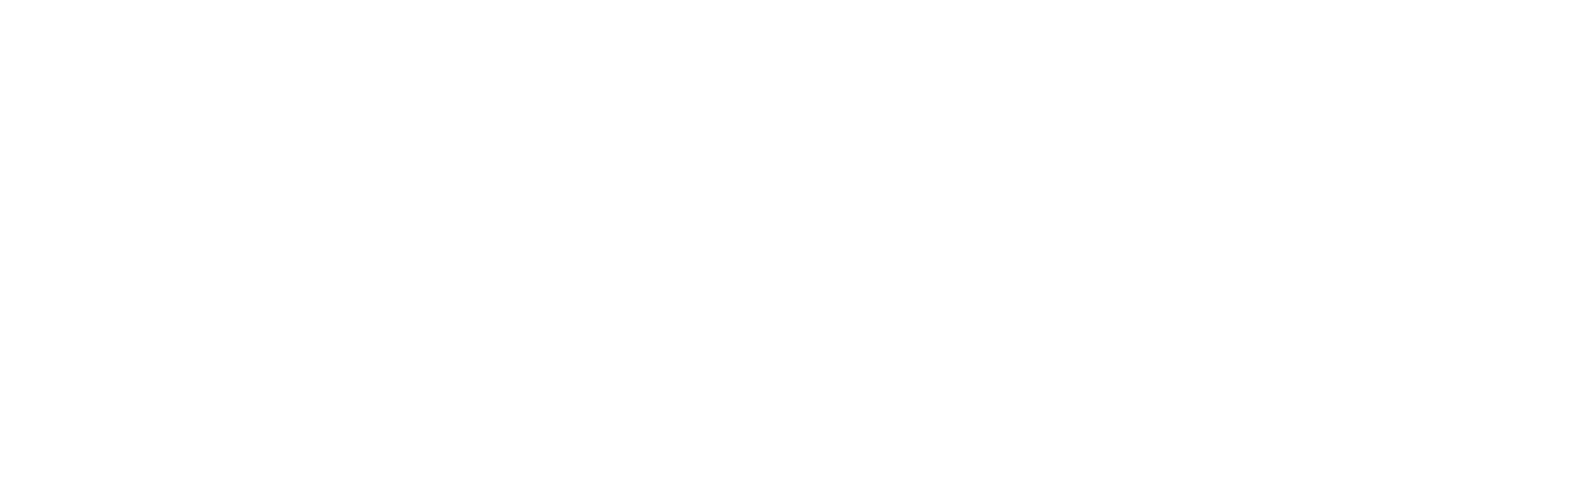
\includegraphics{fig_pdf/UFZ_logo_inv.pdf}}

%%%%%%%%%%%%%%%%%%%%%%%%%%%%%%%%%%%%%%%%%%%%%%%%%%%%%%%%%%%%%%%%%%%%%%%%%%%%%%%%%%%%%%%%%%%%%%%%%%%%%%%
% Optionen für Anmerkungen
\mode<presentation>{%
\setbeameroption{hide notes}				% keine Notizen (default)
%\setbeameroption{show notes}				% Notizen und Frames gemischt
%\setbeameroption{show only notes}			% nur Notizen
%
%\usepackage{pgfpages}					% wird für nachfolgendes benötigt
%\setbeameroption{show notes on second screen=left}	% wie gesagt; left, right, bottom, top
}




%%% DK packages and settings
\usepackage{amsmath}
\usepackage{pgfpages}
\pgfpagesuselayout{resize to}[a4paper, landscape]   % border shrink=5mm
\usepackage{siunitx}  
%\sisetup{locale = DE} 
\usepackage{tikz}
\usepackage{pgfplots}
\usepackage{animate}

\usetikzlibrary{math}
%\usetikzlibrary{datavisualization.formats.functions}
%\usetikzlibrary{datavisualization}
\usetikzlibrary{intersections}
\usepgfplotslibrary{groupplots,dateplot}
\pgfplotsset{compat=1.16}

\tikzset{
%DKspring(length) length=2...10
DKspring/.pic={
\coordinate (half_up) at (0.5*0.125*#1-0.5*0.125*2, 0.5*0.125*10-0.5*0.125*#1); %at (0.5*(#1-0.2), 0.5*(1.0-#1));
\coordinate (full_up)   at ( 0.125*#1-    0.125*2,     0.125*10-    0.125*#1);
\coordinate (full_down) at ( 0.125*#1-    0.125*2,    -0.125*10+    0.125*#1);
\draw (0, 0) -- ++(1, 0) -- ++(half_up)
    -- ++(full_down) -- ++(full_up) 
    -- ++(full_down) -- ++(full_up)
    -- ++(full_down) -- ++(full_up)
    -- ++(full_down) -- ++(half_up)
    -- ++(1, 0);
    },   
%DKdashpot(length) length=02...10    
DKdashpot/.pic={
\coordinate (upper_end) at (#1-0.5, 0.5);
\coordinate (lower_end) at (#1-0.5,-0.5);
\coordinate (upper_pos) at (#1-1, 0.5);
\coordinate (lower_pos) at (#1-1,-0.5);
\coordinate (center_pos) at (#1-1, 0.0);
\coordinate (center_end) at (#1, 0.0);
\draw (0, 0) -- ++(1, 0);
\draw (upper_end) -- (1, 0.5) -- (1, -0.5) -- (lower_end);
\draw (center_pos) -- (center_end);
\draw (upper_pos) -- (lower_pos);
    },
DKbase/.pic={
\draw[thick] (0, 1.5) -- (0, -1.5);
\foreach \y in {-1.5,-1.0,...,1.0} \draw[thin] (0, \y) -- +(-0.5, 0.5);
},
 invisible/.style={opacity=0},
  visible on/.style={alt={#1{}{invisible}}},
  alt/.code args={<#1>#2#3}{%
    \alt<#1>{\pgfkeysalso{#2}}{\pgfkeysalso{#3}} % \pgfkeysalso doesn't change the path
  }
}
\newlength\figH     % to scale tikzplotlib figures
\newlength\figW     % to scale tikzplotlib figures


\setbeamercovered{transparent}
%-----------------Custom footnote---------------
\TUBAFFzstrikttext{D. Kern \TUBAFfztrenner T. Nagel --- Vorlesung Bodendynamik --- Sommersemester 2021 }
%-----------------------------------------------


%%%%%%%%%%%%%%%%%%%%%%%%%%%%%%%%%%%%%%%%%%%%%%%%%%%%%%%%%%%%%%%%%%%%%%%%%%%%%%%%%%%%%%%%%%%%%%%%%%%%%%%
% Daten für die Titelseite:
%
% WICHTIG:	german shortcuts funktionieren nicht!! -> ÄäÖöÜüß verwenden
%		\\ fnkt nur im PM, \newline in AM und PM
%
\TUBAFTitel{Bodendynamik}

\TUBAFUntertitel{Dominik Kern, Thomas Nagel}

\TUBAFAutor[D. Kern | T. Nagel]{Dominik Kern, Thomas Nagel}

\TUBAFDatum[SS21]{Sommersemester 2021}

\TUBAFOrt[IFGT/BOME]{Institut für Geotechnik/Lehrstuhl fuer Bodenmechanik und Grundbau}

\TUBAFTitelseiteerlaeuterung{Lehrstuhl Bodenmechanik \& Grundbau\\Institut für Geotechnik\\[0.5cm]Vorlesung Sommersemester 2021}
	
%\TUBAFTitelseitebilder{
\includegraphics{title_page_pic_.jpg}}
%%%%%%%%%%%%%%%%%%%%%%%%%%%%%%%%%%%%%%%%%%%%%%%%%%%%%%%%%%%%%%%%%%%%%%%%%%%%%%%%%%%%%%%%%%%%%%%%%%%%%%%
% pdf-Infos setzen
\hypersetup{%
	pdfauthor={Dominik Kern},			% wird eigentlich von oben übernommen
	pdftitle={Bodendynamik}	% wird eigentlich von oben übernommen
}
%%%%%%%%%%%%%%%%%%%%%%%%%%%%%%%%%%%%%%%%%%%%%%%%%%%%%%%%%%%%%%%%%%%%%%%%%%%%%%%%%%%%%%%%%%%%%%%%%%%%%%%


\begin{document}
\maketitle

%\section{Grundlagen}
%%%%%%%%%%%%%%%%%%%%%%%%%%%%%%%%%%%%%%%%%%%%%%%%
\section{Mechanisches Bodenverhalten}

\subsection{Dämpfungsmodellierung}
\begin{frame}
\frametitle{Hysteretische Dämpfung}
\begin{itemize}
 \item Kraft-Verschiebungsverlauf von Feder und Dämpfer (viskos, hysteretisch) bei harmonischer Bewegung
 \item Leistungsbilanz des Einmassenschwingers im eingeschwungenen Zustand
\end{itemize}
\vfill

\hfill siehe \textsl{V4a.pdf} (handschriftlich)
\end{frame}

%\subsubsection{Komplexe Rechnung}

\begin{frame}
\frametitle{Erinnerungen an Komplexe Zahlen}
\begin{columns}
        \begin{column}[t]{.3\linewidth}
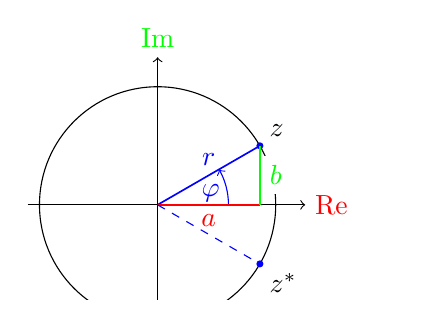
\begin{tikzpicture}[scale=1.5]
\clip (-1.1, -0.8) rectangle (2,1.5);
\coordinate (Null) at (0,0);
\draw[->] (-1.1, 0) -- (1.25, 0) node[right] {\color{red}Re};
\draw[->] (0, -1.1) -- (0, 1.25, 0) node[above] {\color{green}Im};
\draw[name path=Kreis] (0, 0) circle [radius=1];
\path[name path=Strahl] (0, 0) -- (30:1);
\path[name path=kStrahl] (0, 0) -- (-30:1);
\draw[name intersections={of=Kreis and Strahl, by=Zahl}][blue,semithick] (0,0) -- node[above] {$r$} (Zahl);
\fill[blue] (Zahl) circle[radius=0.03];
\draw (Zahl) node[anchor=south west] {$z$};
\draw[blue] (0.45, 0.1) node {$\varphi$};
\draw[blue,->] (0.6, 0) arc [start angle=0, end angle=30, radius=0.6]; 
\draw[red, semithick] (Null) -- node[below, fill=white] {$a$} (Null -| Zahl);
\draw[green, semithick] (Zahl) -- node[right, fill=white] {$b$} (Zahl|- Null);
\draw[name intersections={of=Kreis and kStrahl, by=kZahl}][blue, dashed] (0,0) -- (kZahl);
\draw (kZahl) node[anchor=north west] {$z^*$};
\fill[blue] (kZahl) circle[radius=0.03];
\end{tikzpicture}

         \begin{align*}
          z&={\color{red}a}+i{\color{green}b}={\color{blue}r}e^{i{\color{blue}\varphi}}\\
          z^*&={\color{red}a}-i{\color{green}b}={\color{blue}r}e^{-i{\color{blue}\varphi}}\\
          |z|&=\sqrt{{\color{red}a}^2+{\color{green}b}^2}={\color{blue}r}\\
          \sphericalangle z &=\arctan\frac{\color{green}b}{\color{red}a}={\color{blue}\varphi}
         \end{align*}
        \end{column}
        \begin{column}[t]{.7\linewidth}
        \vspace{-3cm}
        \begin{align*}
         \mathrm{Re}\{z\}&={\color{red}a}  ={\color{blue}r}\cos{\color{blue}\varphi}\\
         \mathrm{Im}\{z\}&={\color{green}b}={\color{blue}r}\sin{\color{blue}\varphi}
        \end{align*}
        \hspace{2cm} Ausgewählte Formeln
         \begin{align*}
          z+z^*&=2\,\mathrm{Re}\{z\}\\
          z_1z_2&=r_1r_2 e^{i(\varphi_1+\varphi_2)}\\
          (z_1z_2^*)^*&=z_1^*z_2\\
          (z_1 z_2)^*&=z_1^*z_2^*\\
          \frac{1}{a+ib}&=\frac{a}{a^2+b^2}-\frac{ib}{a^2+b^2}
         \end{align*}
        \end{column}
\end{columns}
\end{frame}


\begin{frame}
\frametitle{Frequenzgang 1/2}
Komplexe Erweiterung (Re ``sichtbar'', Im ``mitschleppen'')
\hspace{1cm}
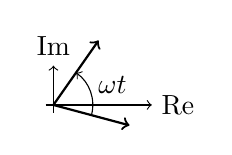
\begin{tikzpicture}[baseline=-1mm]
\draw[->] (-0.1, 0) -- (1.25, 0) node[right] {Re};
\draw[->] (0, -0.1) -- (0, 0.5, 0) node[above] {Im};
\draw[thick,->] (0,0) -- (55: 1); 
\draw[thick,->] (0,0) -- (-15: 1);
\draw[->] (-15:0.5) arc [start angle=-15, end angle=55, radius=0.5];
\draw (0.75, 0.25) node {$\omega t$};
\end{tikzpicture}

\begin{align*}
 u(t)&= \hat{u}\,e^{i\omega t} &\qquad & \text{mit} \qquad &\hat{u}&=r_u e^{-i\psi_u},\\
 a(t)&=\hat{a}\,e^{i\omega t} &\qquad & \text{mit} \qquad &\hat{a}&=r_a e^{-i\psi_a},\\
 F(t)&= \hat{F}\,e^{i\omega t} &\qquad & \text{mit} \qquad &\hat{F}&=r_F e^{-i\psi_F}.
\end{align*}
Standardform des erregten, (viskos) gedämpften Einmassenschwingers
\begin{equation*}
 \ddot{u}+2\zeta\omega_0 \dot{u}+\omega_0^2 u = \omega_0^2\hat{a}\,e^{i\omega t}.
\end{equation*}
Ansatz vom Typ der rechten Seite
\begin{align*}
 -\omega^2 \hat{u}\,e^{i\omega t} +2i\zeta\omega_0\omega \hat{u}\,e^{i\omega t} +\omega_0^2  \hat{u}\,e^{i\omega t} &= \omega_0^2\hat{a}\,e^{i\omega t},\\
 \left(-\eta^2 + 2i\zeta\eta +1 \right)\hat{u}\,e^{i\omega t}&= \hat{a}\,e^{i\omega t}.
\end{align*}
\end{frame}

\begin{frame}
\frametitle{Frequenzgang 2/2} 
\hfill
 $\hat{u}=\underbrace{\frac{1}{1-\eta^2 + 2i\zeta\eta}}_{H(\eta)} \hat{a}$
\hfill 
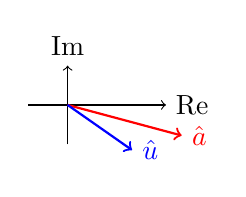
\begin{tikzpicture}[baseline=0mm]
\draw[->] (-0.5, 0) -- (1.25, 0) node[right] {Re};
\draw[->] (0, -0.5) -- (0, 0.5, 0) node[above] {Im};
\draw[thick,red,->] (0,0) -- (-15: 1.5) node[right] {$\hat{a}$};
\draw[thick,blue,->] (0,0) -- (-35: 1) node[right] {$\hat{u}$};
\end{tikzpicture}


Der Frequenzgang $H(\eta)$ enthält sowohl die Vergrößerungsfunktion $V$ 
als auch die Phasendifferenz $\psi$
\only<1>{
\begin{align*}
V=|H|&=\left|\frac{1-\eta^2}{(1-\eta^2)^2 + (2\zeta\eta)^2}-
\frac{2i\eta\zeta}{(1-\eta^2)^2 + (2\zeta\eta)^2}\right| \\
 &= \sqrt{\frac{(1-\eta^2)^2+(2\eta\zeta)^2}{\Bigl((1-\eta^2)^2 + (2\zeta\eta)^2\Bigr)^2}}\\
 &= \sqrt{\frac{1}{(1-\eta^2)^2 + (2\zeta\eta)^2}}
\end{align*}
}
\only<2>{
\begin{align*}
\psi=-\,\sphericalangle H &=-\,\sphericalangle \left\{\frac{1-\eta^2}{(1-\eta^2)^2 + (2\zeta\eta)^2}-
\frac{2i\eta\zeta}{(1-\eta^2)^2 + (2\zeta\eta)^2}\right\}\\
&=-\arctan\left(\frac{-2\eta\zeta}{1-\eta^2}\right)
=\arctan\left(\frac{2\eta\zeta}{1-\eta^2}\right)
\end{align*}

\vfill
\alert{\textbf{HA}: Was ändert sich für hysteretische Dämpfung?}
}
\end{frame}


\begin{frame}
\frametitle{Leistungsbilanz{\normalsize-- Grenzfälle} }
\begin{columns}
        \begin{column}[t]{.5\linewidth}
        \hspace{9mm} Energiespeicher
        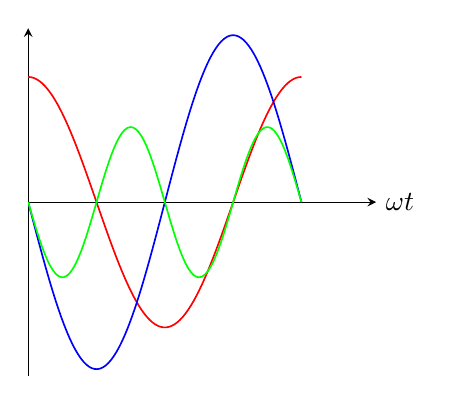
\begin{tikzpicture}
\begin{axis}[
    width=6cm, 
    height=6cm,
    axis x line=center, 
    axis y line=middle, 
    xlabel={$\omega t$},
     x label style={at={(current axis.right of origin)}, right},
    samples=100,
    ymin=-1.25, ymax=1.25,
    xmin=0, xmax=8,
    domain=0.0*pi:2*pi,
    ticks=none
]
\addplot [mark=none, semithick, red] {0.9*cos(deg(x))};
\addplot [mark=none, semithick, blue] {-1.2*sin(deg(x))};
\addplot [mark=none, semithick, green] {-1.2*sin(deg(x))*0.9*cos(deg(x))};
\end{axis}
\end{tikzpicture}  

\bigskip

         Federkraft {\color{red}$F_F$},\\ 
         Geschwindigkeit {\color{blue}$\dot{u}$} und\\
         Momentanleistung {\color{green}$P_F$}
        \end{column}
        \begin{column}[t]{.5\linewidth}
        \hspace{7mm} Energiequelle/-senke
        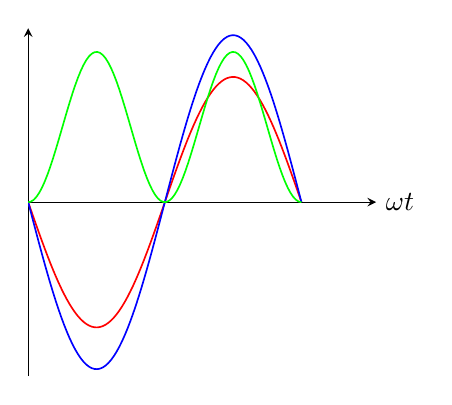
\begin{tikzpicture}
\begin{axis}[
    width=6cm, 
    height=6cm,
    axis x line=center, 
    axis y line=middle, 
    xlabel={$\omega t$},
     x label style={at={(current axis.right of origin)}, right},
    samples=100,
    ymin=-1.25, ymax=1.25,
    xmin=0, xmax=8,
    domain=0.0*pi:2*pi,
    ticks=none
]
\addplot [mark=none, semithick, red] {-0.9*sin(deg(x))};
\addplot [mark=none, semithick, blue] {-1.2*sin(deg(x))};
\addplot [mark=none, semithick, green] {1.2*sin(deg(x))*0.9*sin(deg(x))};
\end{axis}
\end{tikzpicture}      

        \bigskip

         Dämpferkraft {\color{red}$F_D$},\\ 
         Geschwindigkeit {\color{blue}$\dot{u}$} und\\
         Momentanleistung {\color{green}$P_D$}         
\end{column}
\end{columns}
\end{frame}

\begin{frame}
\frametitle{Leistungsbilanz {\normalsize -- Einmassenschwinger 1/3}}
\begin{columns}
        \begin{column}[t]{.5\linewidth}
        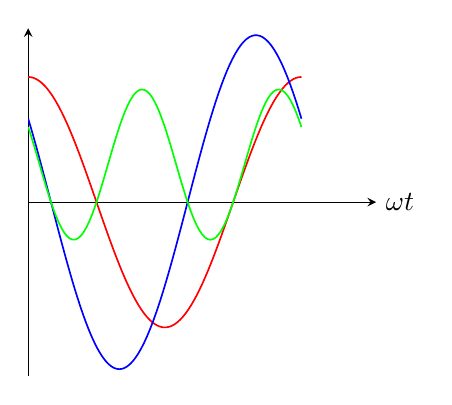
\begin{tikzpicture}
\begin{axis}[
    width=6cm, 
    height=6cm,
    axis x line=center, 
    axis y line=middle, 
    xlabel={$\omega t$},
     x label style={at={(current axis.right of origin)}, right},
    samples=100,
    ymin=-1.25, ymax=1.25,
    xmin=0, xmax=8,
    domain=0.0*pi:2*pi,
    ticks=none
]
\addplot [mark=none, semithick, red] {0.9*cos(deg(x))};
\addplot [mark=none, semithick, blue] {1.2*cos(deg(x)+60)};
\addplot [mark=none, semithick, green] {1.2*cos(deg(x)+60)*0.9*cos(deg(x))};
\end{axis}
\end{tikzpicture} 
     
\bigskip

         Anregende Kraft {\color{red}$F$},\\ 
         Geschwindigkeit {\color{blue}$\dot{u}$} und\\
         Momentanleistung {\color{green}$P$}
        \end{column}
        \begin{column}[t]{.5\linewidth}
        \vspace{-4.5cm}
\begin{align*}
 F&=r_F\,e^{i(\omega t-\psi_a)} \\
 u&=r_u\,e^{i(\omega t-\psi_u)} \\
  &=r_u\,e^{i(\omega t-\psi_a-\psi)} \\
 v&=i\omega r_u\,e^{i(\omega t-\psi_a-\psi)}\\
 &=\omega r_u\, e^{i\frac{\pi}{2}} e^{i(\omega t-\psi_a-\psi)}\\
 & =\omega r_u \,e^{i\left(\omega t+\frac{\pi}{2}-\psi_a-\psi\right)}\\
 r_v&=\omega r_u \\
 \psi_v&=\psi_a+\psi-\frac{\pi}{2}
 \end{align*}
\end{column}
\end{columns}
\end{frame}

\begin{frame}
\frametitle{Leistungsbilanz {\normalsize -- Einmassenschwinger 2/3}}
 \begin{align*}
  P&=\mathrm{Re}\left\{F \right\}\mathrm{Re}\left\{v\right\}\\
  &=\frac{1}{2}(F+F^*)\frac{1}{2}(v+v^*)\\
  &=\frac{1}{4}\bigl(Fv+Fv^*+F^*v+F^*v^*\bigr)=\frac{1}{4}\Bigl(Fv+Fv^*+(Fv+Fv^*)^*\Bigr)\\
  &=\frac{1}{2}\mathrm{Re}\left\{Fv+Fv^*\right\}\\
  &=\frac{1}{2}\mathrm{Re}\left\{r_F\,e^{i(\omega t-\psi_a)} r_v\,e^{i(\omega t-\psi_v)}
  +r_F\,e^{i(\omega t-\psi_a)} r_v\,e^{-i(\omega t-\psi_v)} \right\}\\
  &=\mathrm{Re}\left\{\frac{r_F r_v}{2}e^{i(\psi_v-\psi_a)}
  \bigl( e^{i2(\omega t - \psi_v)} + 1  \bigr)
   \right\}\\
 \end{align*}

\end{frame}

\begin{frame}
\frametitle{Leistungsbilanz {\normalsize -- Einmassenschwinger 3/3}}
\begin{equation*}
   P=\mathrm{Re}\left\{P_S
  \bigl( e^{i2(\omega t - \psi_v)} + 1  \bigr) \right\} 
  \qquad
  \text{mit}
  \qquad
  P_S=\frac{r_F r_v}{2}e^{i(\psi_v-\psi_a)}
\end{equation*}
Formelsammlung: \quad $\mathrm{Re}\{z_1 z_2\}=\mathrm{Re}\{z_1\}\mathrm{Re}\{z_2\} - \mathrm{Im}\{z_1\}\mathrm{Im}\{z_2\}$
\begin{align*}
   P&=\mathrm{Re}\left\{P_S\right\}\mathrm{Re}\left\{ e^{i2(\omega t - \psi_v)} + 1  \right\}
   -\mathrm{Im}\left\{P_S\right\}\mathrm{Im}\left\{ e^{i2(\omega t - \psi_v)} + 1  \right\}\\
   &=\mathrm{Re}\left\{P_S\right\}\Bigl( \cos(2\omega t - 2\psi_v) + 1 \Bigl)
   -\mathrm{Im}\left\{P_S \right\} \sin(2\omega t- 2\psi_v)
\end{align*}
Damit ist die Momentleistung (Scheinleistung $|P_S|$) dargestellt als Summe eines schwellenden Verlaufs (Wirkleistung $\mathrm{Re}\left\{P_S\right\}$) und eines mittelwertfreien Verlaufs (Blindleistung $\mathrm{Im}\left\{P_S \right\}$). 

\end{frame}

%%%%%%%%%%%%%%%%%%%%%%%%%%%%%%%%%%%%%%%%%%%%%%%%

\subsection{Zyklische Belastung}

\begin{frame}
\frametitle{Szenarien}

\begin{tabular}{ll} 
%\toprule
\textbf{Erdbeben} & \textbf{Technische Vorgänge (Maschinen, Verkehr)} \\[2mm] 
%\midrule 
breites Frequenzspektrum  & diskretes Frequenzspektrum  \\[1mm] 
niedrige Frequenzen& hohe Frequenzen\\
($0.5 \dots 10$\,Hz)  & (bis kHz-Bereich) \\[1mm] 
wenige Sekunden  & langanhaltend \\[1mm] 
wenige Zyklen & viele Zyklen \\[1mm] 
verschiebungsgesteuert & kraftgesteuert \\[1mm] 
große Verformungen& kleine Verformungen\\
(starke Erdbeben) & (Normalbetrieb) 
%\bottomrule
\end{tabular}

\end{frame}

\begin{frame}
\frametitle{Begriffe}
Als \textsl{zyklisch} werden diejenigen wiederholten Belastungen definiert, 
bei denen Trägheitseffekte vernachlässigt werden können, andernfalls werden sie als
\textsl{transient} oder \textsl{dynamisch} bezeichnet.

\bigskip

\textsl{Nichtlineares} Verhalten tritt in den meisten Böden auf, 
sobald die Dehnungen größer als ca. $\varepsilon=10^{-5}$ werden. 

\bigskip

Das nichtlineare Verhalten von Böden unter zyklischer Belastung ist kompliziert 
und soll zunächst nur phänomenologisch beschrieben werden.
\end{frame}

\begin{frame}
\frametitle{Dehnungsgesteuerte Belastung}
\begin{figure}
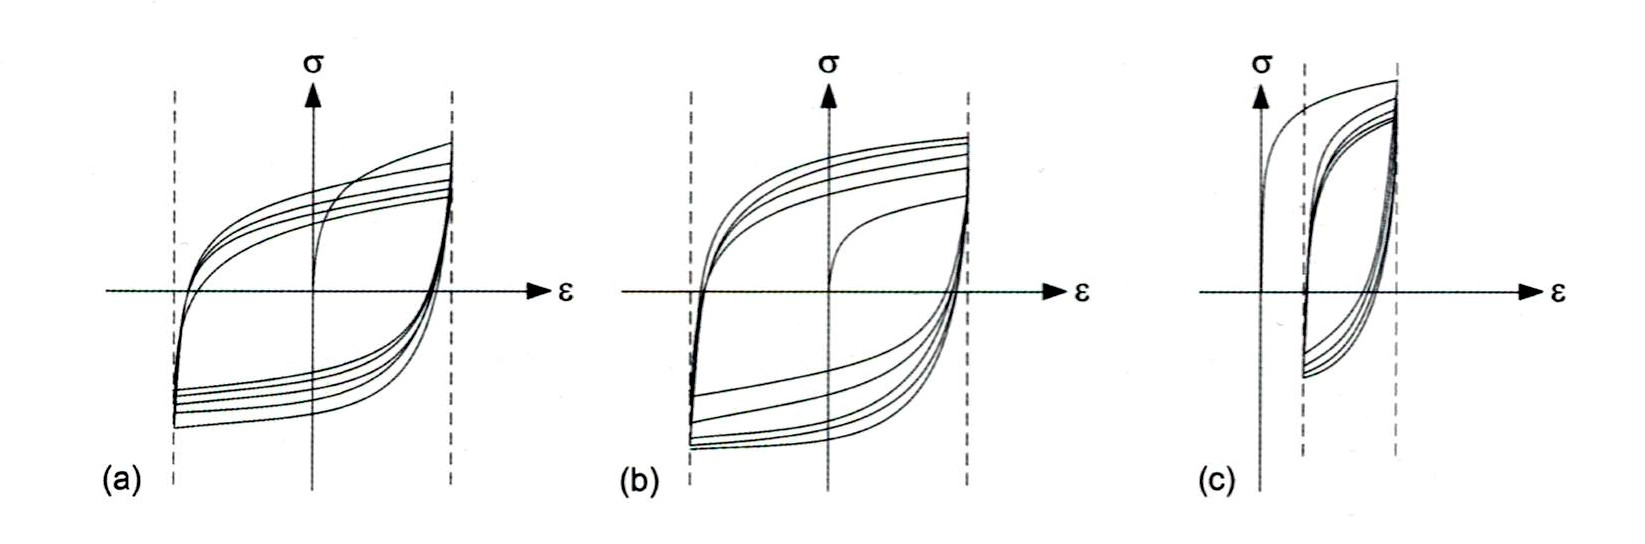
\includegraphics[width=\linewidth]{fig_img/bild14abc.jpg}
\caption*{(a) Entfestigung, (b) Verfestigung, (c) Relaxation der Mittelspannung \cite{Vrettos2017}} 
\end{figure}
Das Verhalten ist vorwiegend durch die Vorgeschichte bestimmt.
\end{frame}

\begin{frame}
\frametitle{Spannungsgesteuerte Belastung}
\begin{figure}
\centering
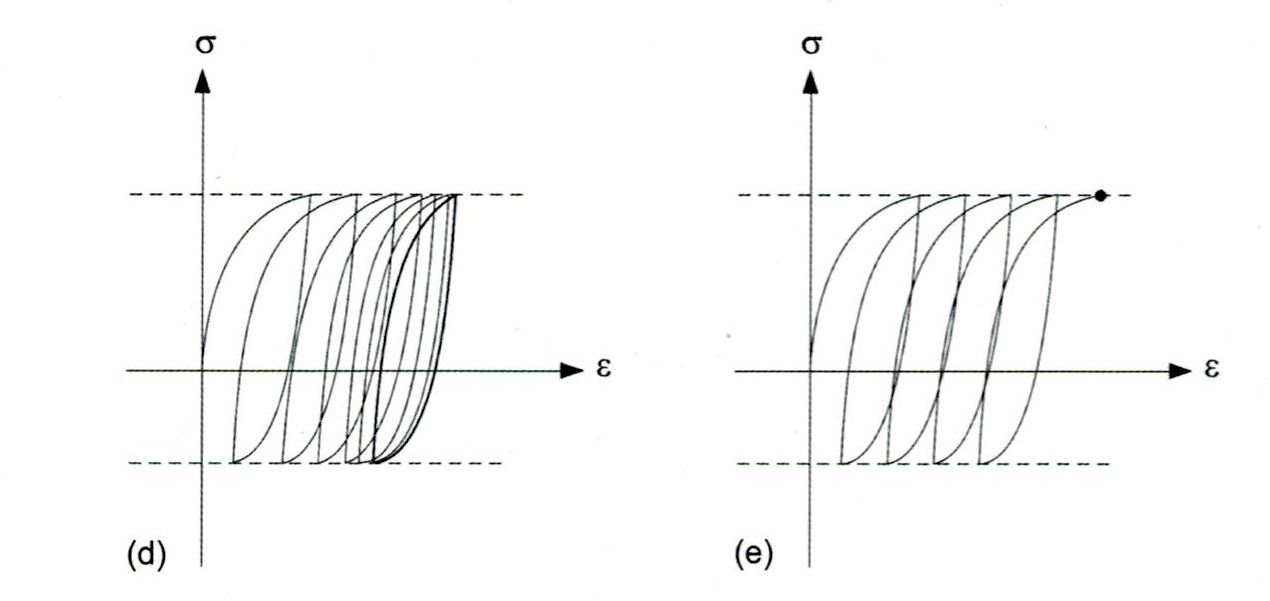
\includegraphics[width=0.75\linewidth]{fig_img/bild14de.jpg}
\caption*{(d) Einspielen (Shakedown), (e) unbegrenztes Anwachsen plastischer Dehnungen (inkrementeller Kollaps) \cite{Vrettos2017}} 
\end{figure}
Einspielen tritt eher bei teilweise gesättigten Böden und unter dränierten Verhältnissen auf, das unbegrente Anwachsen eher bei gesättigten Böden.
\end{frame}

\begin{frame}
\frametitle{Stationärer Zustand}
\begin{figure}
\centering
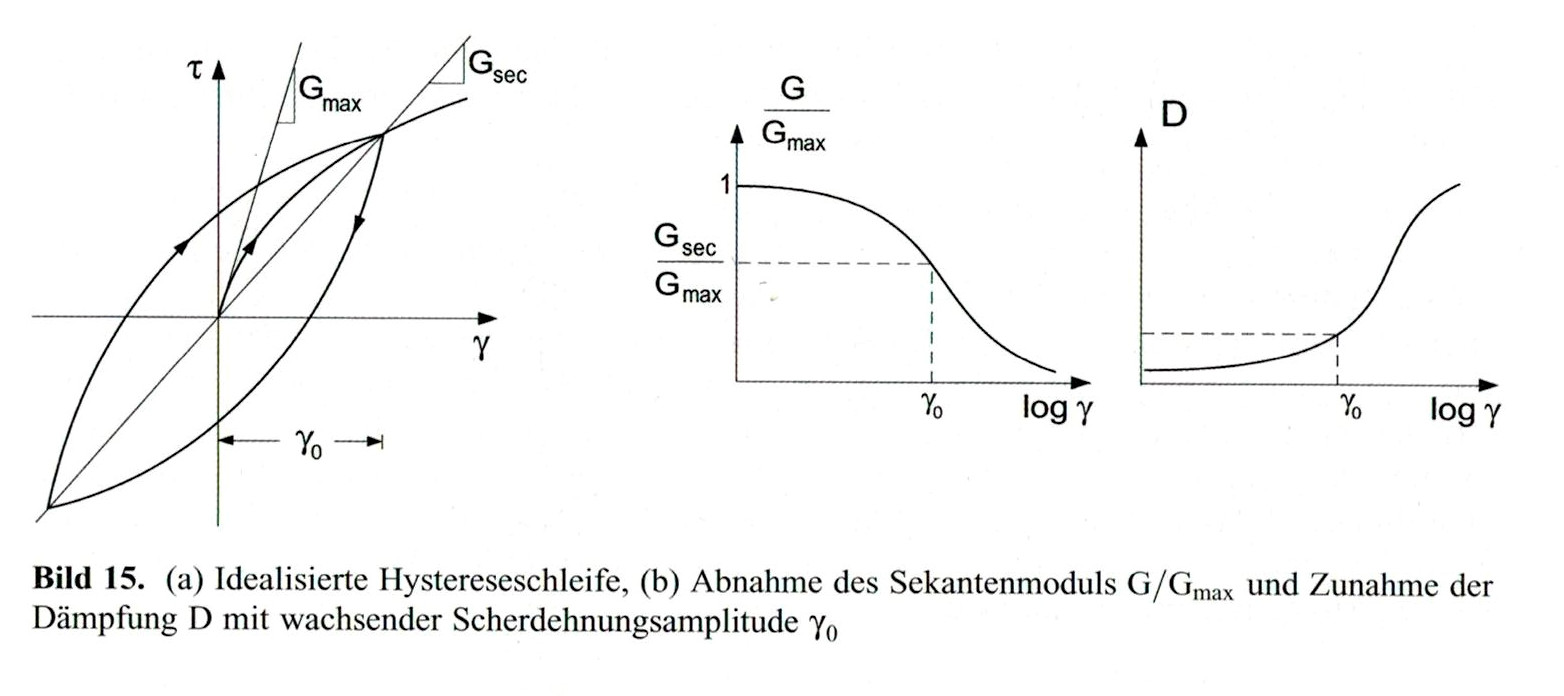
\includegraphics[width=\linewidth]{fig_img/bild15.jpg}
\caption*{Solange keine plastischen Verformungen gesucht werden,
wird angenommen, dass sich ein stationärer Zustand nach einigen Lastzyklen eingestellt hat \cite{Vrettos2017}.} 
\end{figure}
\end{frame}


\begin{frame}
\frametitle{Parameterabhängigkeit}
\begin{columns}
\begin{column}[t]{.475\linewidth}
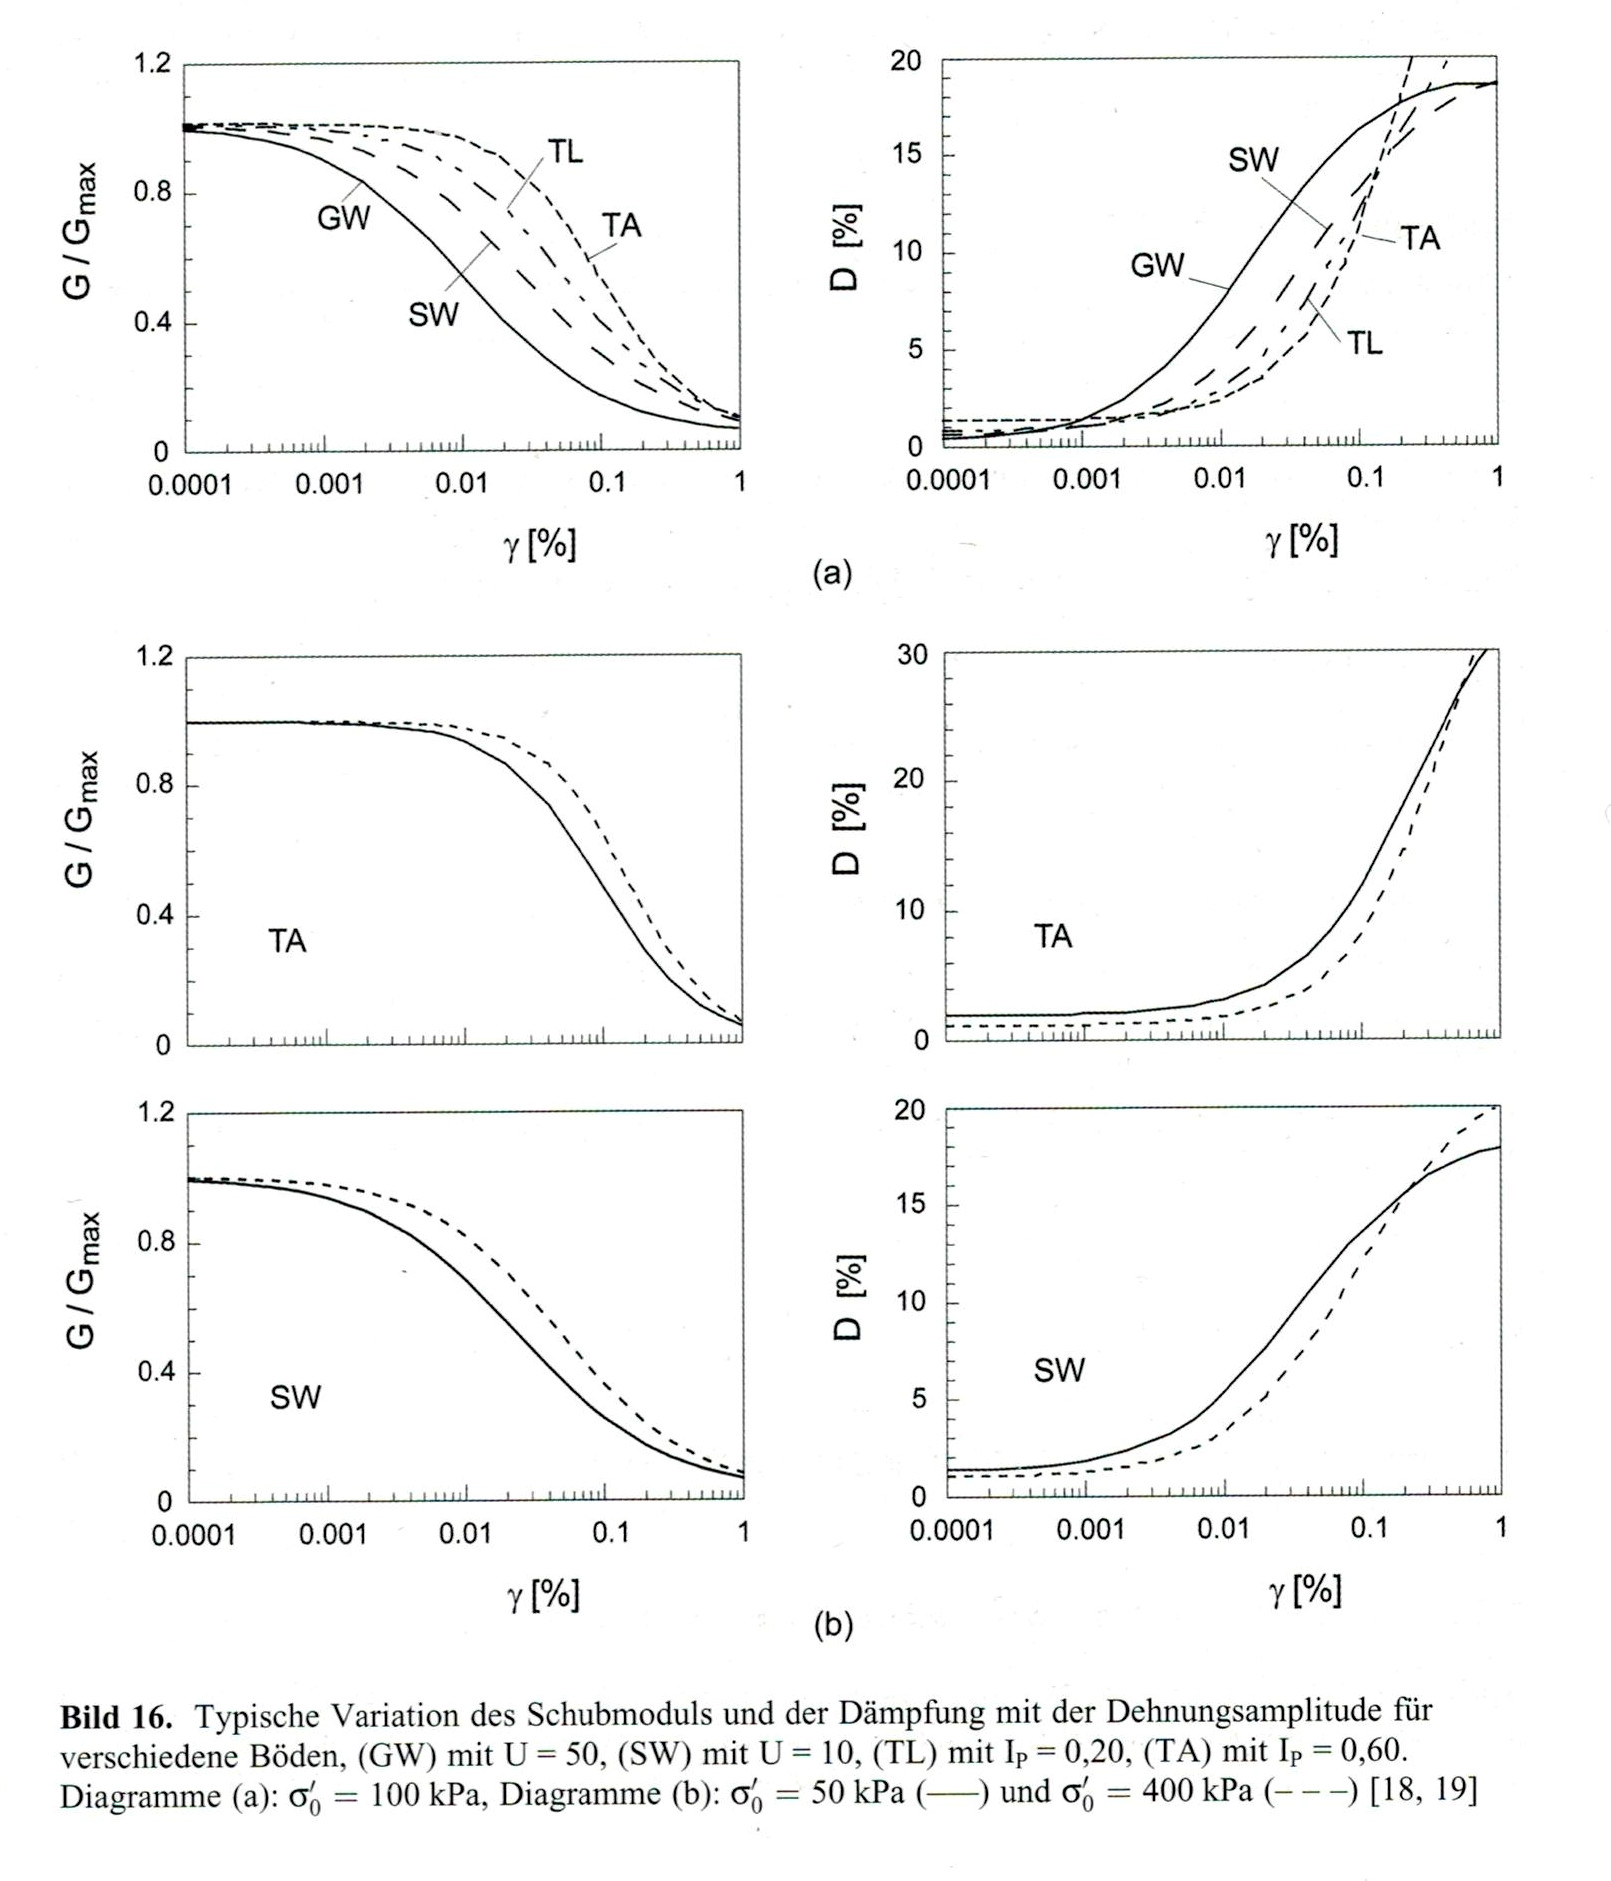
\includegraphics[width=\linewidth]{fig_img/bild16.jpg}
\end{column}
\begin{column}[t]{.525\linewidth}
\vspace{-5cm}

Schubmodul und Dämpfung werden -- außer von der Dehnungsamplitude -- vornehmlich von folgenden Parametern beeinflusst: effektives Druckniveau, Porenzahl, Plastizitätszahl, Überkonsolidierungsgrad bei bindigen Böden sowie Anzahl der Zyklen \cite{Vrettos2017}.
\end{column}
\end{columns}
\end{frame}

\begin{frame}
\frametitle{Einfache hysteretische Modelle}
\begin{figure}
\centering
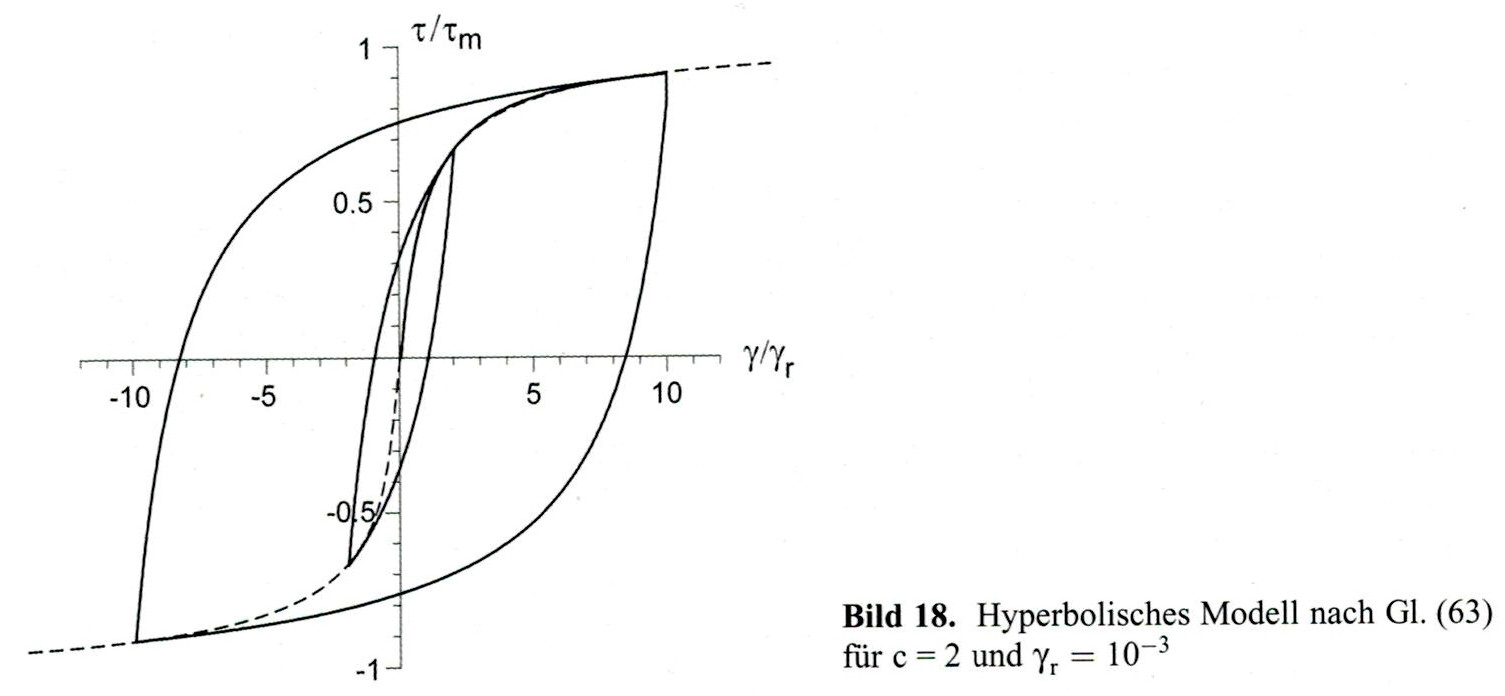
\includegraphics[width=0.95\linewidth]{fig_img/bild18.jpg}
\caption*{Gleichung (61) beschreibt die Skeleton-Kurve (gestrichelt)
und Gleichung (63) die Konstruktion der Spannungs-Dehnungsbeziehung
\cite{Vrettos2017}.} 
\end{figure}
\end{frame}

\begin{frame}
\frametitle{Einfache hysteretische Modelle}
Zur Beschreibung des Bodenverhaltens stehen grundsätzlich zwei Alternativen zur Auswahl \cite{Vrettos2017}:
\begin{itemize}
 \item Entwicklung eines Modells, womit das hysteretisch-plastische Stoffverhalten innerhalb jedes Belastungszyklus beschrieben wird. 
 \item Aufstellung eines empirischen Akkumulationsmodells, das die wesentlichen Parameter beinhaltet, ohne jedoch die Vorgänge in jedem Zyklus zu beschreiben.
\end{itemize}
\end{frame}

\begin{frame}
\frametitle{Zusatzmaterial} % online courses
\vfill
\begin{center}

\includegraphics[width=0.2\textwidth]{fig_img/youtube.png}  

\href{https://www.youtube.com/watch?v=01_KWg3QriE}{\textsl{Office Hours: CEEN 545 - Lecture 18 - Dynamic Soil Properties (Part 1)}}

\href{https://www.youtube.com/watch?v=Mngr3tujIjM}{\textsl{Office Hours: CEEN 545 - Lecture 19 - Dynamic Soil Properties (Part 2)}}
\end{center}  
\vfill
Die Reihenfolge der Videos (Teil 1: Experimentelle Parameterbestimmung, Teil 2: Mathematische Modelle) ist andersrum als in dieser Vorlesung und enthält einige Vorgriffe, nichtsdestotrotz lohnt sich schon jetzt ein Blick in Teil 2.

\end{frame}



%%%%%%%%%%%%%%%%%%%%%%%%%%%%%%%%%%%%%%%%%%%%%%%%

\section*{Literaturverzeichnis}

\begin{frame}[allowframebreaks]{}
	\printbibliography
\end{frame}
\end{document}
